\section{Código de ejemplo de una aplicación}

A continuación exponemos brevemente el código de una aplicación que se encuentra en el repositorio en GitHub de aplicaciones plantilla para Google Cast. Esta aplicación sirve para enviar texto desde una pestaña de Google Chrome y mostrarlo en una pantalla conectada a un Chromecast.

\

Esta \href{https://github.com/googlecast/CastHelloText-chrome}{aplicación} consta de dos partes: la del emisor (Google Chrome) y la del receptor (Chromecast).
Ambas son web apps en HTML que cargan un código JavaScript.
Para ejecutarla debemos alojarla en un servidor.

\begin{figure}[H]
	\centering
	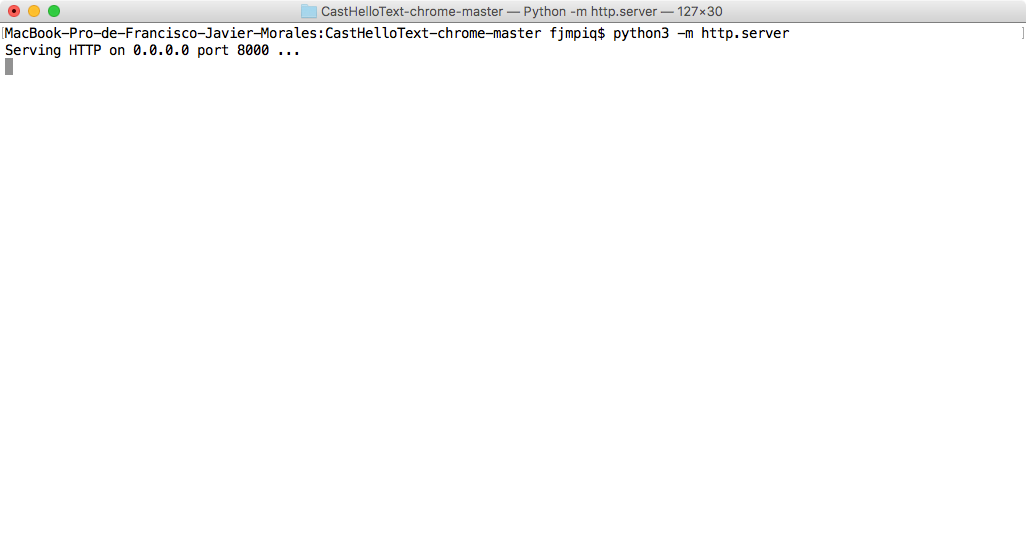
\includegraphics[width=1.1\textwidth]{./Imagenes/creando_servidor.png}
	\label{fig:fondo}
	\caption{Creando un servidor en el puerto 8000}
\end{figure}

Desde Chrome, accedemos a la aplicación emisora (chromehellotext.html).

\begin{figure}[H]
	\centering
	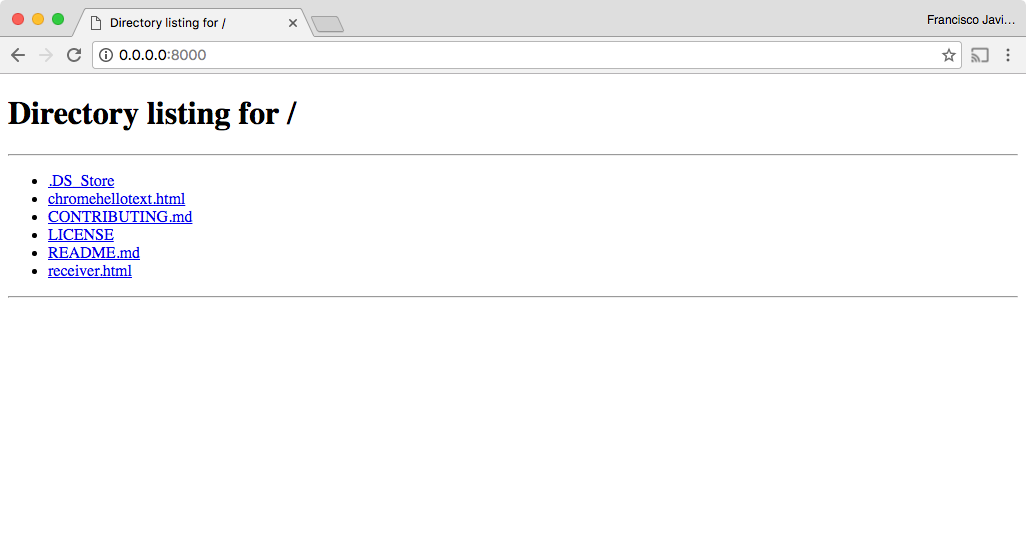
\includegraphics[width=1.1\textwidth]{./Imagenes/directorylisting.png}
	\label{fig:fondo}
	\caption{Listado del directorio del servidor que acabamos de crear}
\end{figure}

\begin{figure}[H]
	\centering
	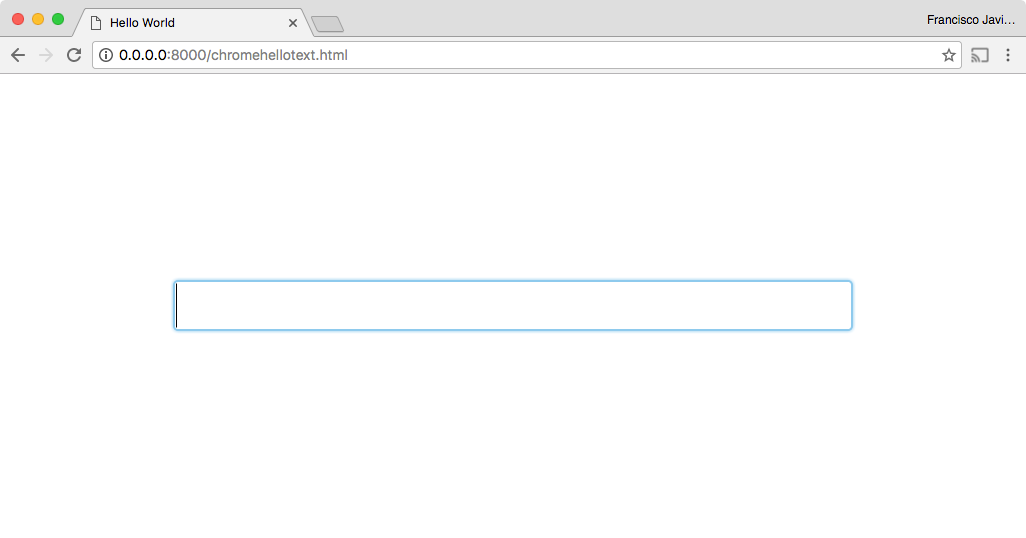
\includegraphics[width=1.1\textwidth]{./Imagenes/emisor1.png}
	\label{fig:fondo}
	\caption{Aplicación emisora}
\end{figure}

A continuación, desde la extensión de Google Cast, seleccionamos enviar el contenido de la aplicación a nuestro Chromecast.

\begin{figure}[H]
	\centering
	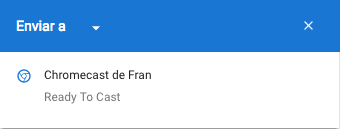
\includegraphics[width=0.7\textwidth]{./Imagenes/seleccion.png}
	\label{fig:fondo}
	\caption{Selección del Chromecast}
\end{figure}


En ese momento, debería cargar en el Chromecast la aplicación receptora (receiver.html).
Ya podemos escribir texto en el emisor y, al pulsar intro, debería aparecer en el televisor.


\begin{figure}[H]
	\centering
	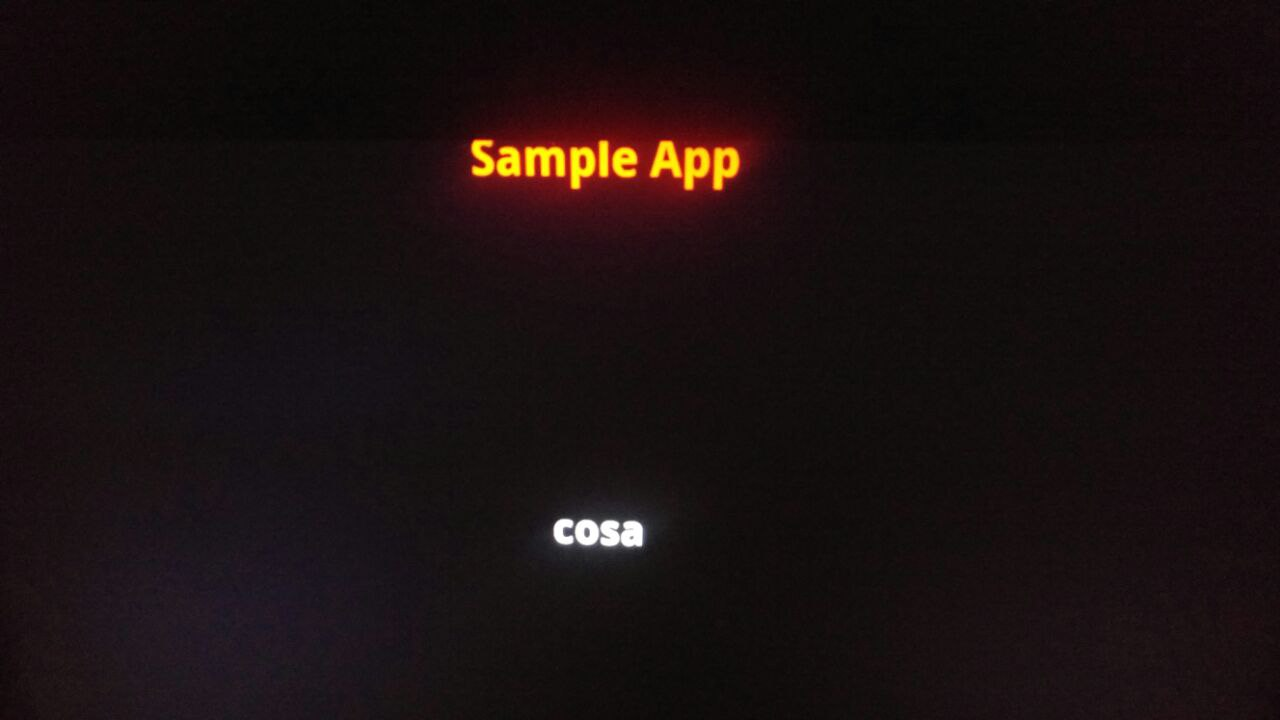
\includegraphics[width=1\textwidth]{./Imagenes/receptor.jpg}
	\caption{Televisión recibiendo mensajes}
\end{figure}
	

Para enviar vídeo podríamos usar esta otra \href{https://github.com/googlecast/CastHelloVideo-chrome}{aplicación}.